\subsection{Classification of Flow}
Much like we did with linear systems in the plane, we want to classify all (possibly non-linear) systems in any number of dimensions. This as daunting a task as it sounds. At the very least, we first need to start with how this classification will work, namely when can we say that two flows are `the same'? This leads us to the notion of similarity.

We will say that two flows $\Phi$ and $\Psi$ are similar (or more precisely conjugate) when there is a bijection $h$ such that
$$ h^{-1} \circ \Phi \circ h = \Psi$$
\begin{remark}
    Note how similar this is to similarity of matrices: we say two matrices $A, B$ are similar if there is an invertible $T$ such that $T^{-1}AT = B$.
\end{remark}
Note how we have not made any assumption about $h$ being continuous/differentiable/smooth/etc. Such assumptions can vary based on the field of study. Taking $h$ to be a homeomorphism is quite common (and as we will show, somewhat easy to achieve). If $h$ is indeed just a homeomorphism, we say we have \textit{topological conjugacy}. Getting $h$ to be a diffeomorphism is much nicer, but also a lot harder.\\

Now that we have the general overview, let's try and be a bit more precise. Suppose $x$ is a solution to the non-linear system
\begin{align*}
    x' &= f(x)\\
    x(0) &= v
\end{align*}
and $z$ is its linearization. In other words, $z$ is the solution to
\begin{align*}
    z'(t) &= Df(x(t)) z\\
    z(0) &= w
\end{align*}
(where $w$ is taken to be small). 
As we've discussed, $x + z$ is an approximation solution to $x' = f(x)$ with $x(0) = v + w$ (this is exactly \autoref{prop:approx-solns}). Thus we would like to say that $x$ is conjugate to $x + z$. Unfortunately in general this is not true, even in the simplest case where we approximate near a steady state. Consider the following example.

\subsubsection{Example 1}
Suppose we are given the differential equation
$$ \matrix{x\\y}' = \matrix{x^2 \\ y^2} $$
Clearly, the only equilibrium point is the origin and 
$$ Df(0, 0) = \matrix{0 & 0\\0 & 0} $$
Thus the linearised system has constant solutions. And indeed, if we were to look in a small neighbourhood near the origin the solutions (on a small time interval) do look roughly constant (see \href{https://anvaka.github.io/fieldplay/?dt=0.02&fo=0.995&dp=0.009&cm=1&cx=-0.05585000000000001&cy=0.0063499999999999945&w=1.0917&h=1.0917&vf=\%2F\%2F\%20p.x\%20and\%20p.y\%20are\%20current\%20coordinates\%0A\%2F\%2F\%20v.x\%20and\%20v.y\%20is\%20a\%20velocity\%20at\%20point\%20p\%0Avec2\%20get_velocity\%28vec2\%20p\%29\%20\%7B\%0A\%20\%20vec2\%20v\%20\%3D\%20vec2\%280.\%2C\%200.\%29\%3B\%0A\%0A\%20\%20\%2F\%2F\%20change\%20this\%20to\%20get\%20a\%20new\%20vector\%20field\%0A\%20\%20v.x\%20\%3D\%20p.x\%20*\%20p.x\%3B\%0A\%20\%20v.y\%20\%3D\%20p.y\%20*\%20p.y\%3B\%0A\%0A\%20\%20return\%20v\%3B\%0A\%7D&pc=10000&code=\%2F\%2F\%20p.x\%20and\%20p.y\%20are\%20current\%20coordinates\%0A\%2F\%2F\%20v.x\%20and\%20v.y\%20is\%20a\%20velocity\%20at\%20point\%20p\%0Avec2\%20get_velocity\%28vec2\%20p\%29\%20\%7B\%0A\%20\%20vec2\%20v\%20\%3D\%20vec2\%280.\%2C\%200.\%29\%3B\%0A\%0A\%20\%20\%2F\%2F\%20change\%20this\%20to\%20get\%20a\%20new\%20vector\%20field\%0A\%20\%20v.x\%20\%3D\%20p.x\%20*\%20p.x\%3B\%0A\%20\%20v.y\%20\%3D\%20p.y\%20*\%20p.y\%3B\%0A\%0A\%20\%20return\%20v\%3B\%0A\%7D}{here}). However, and this is the key, the constant solution is \textit{not} conjugate to the non-linear system. Intuition is enough to guide us here: if the flow of a system is constant, then there is no motion. We really should not consider this equivalent to a system that does have motion. It might be a useful exercise to prove to yourself that constant systems cannot be conjugate to non-constant ones, before I do that right now.

Quite simply, the key is that if the solutions to a system are constant then the flow map $\Phi_t$ is simply the identity for all $t$. Thus $h \circ \Phi_t \circ h^{-1}$ must be the identity as well.\\


Neverthenonetheless, there will be cases where we \textit{do} get conjugacy, as in the following example.

\subsubsection{Example 2}
Consider the system
\begin{align*}
    x' &= x + y^2\\
    y' &= -y
\end{align*}
Then $f(x, y) = (x + y^2, -y)$. Clearly we have only one equilibrium point, which is at the origin again. Thus the linearisation around it is given by
$$ \matrix{x\\y}' = \underbrace{\matrix{1 & 0\\0 & -1}}_A \matrix{x\\y} $$
Without any further work, we can conclude that the linearised system is unstable and has a saddle. Note that if $y$ is small, then $y^2$ would be even smaller. Thus we would expect the non-linear system to look quite similar to its linearisation around the origin.

\begin{figure}[h]
    \centering
    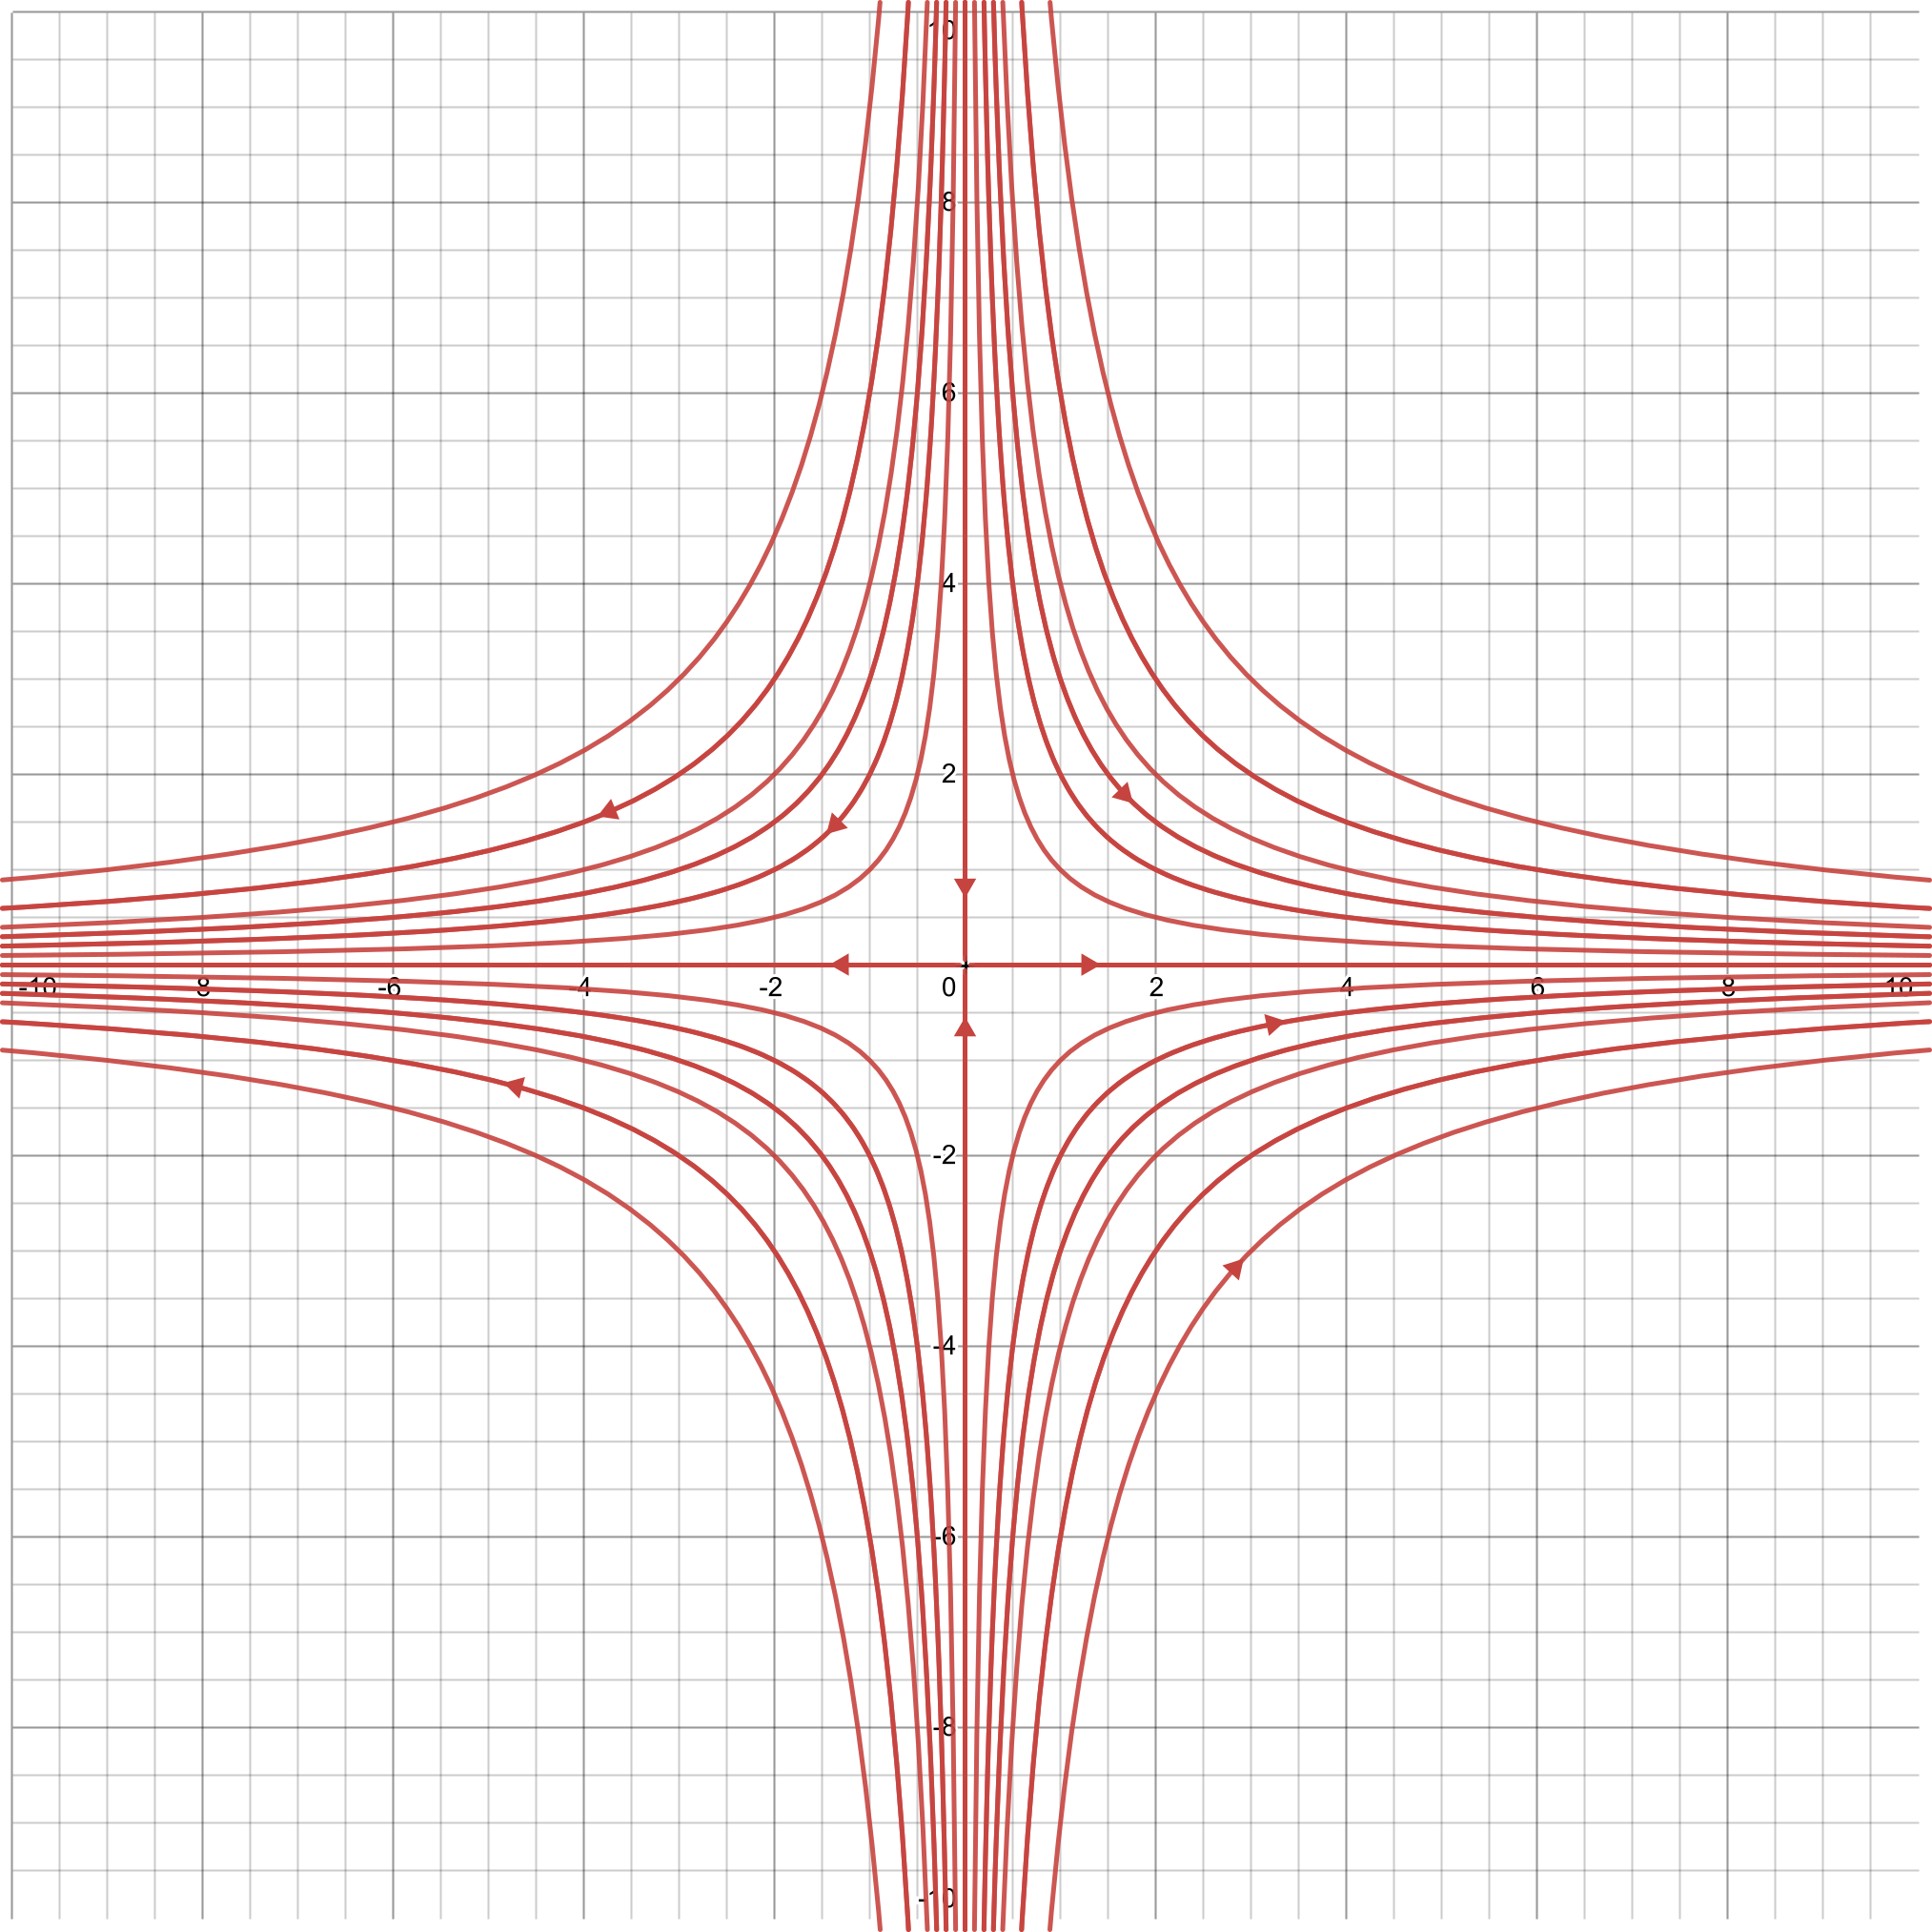
\includegraphics[scale=0.17]{Images/linearisation_eg1.png}
    \caption{Phase portrait of linearised system, \href{https://www.desmos.com/calculator/jqmz5jddc4}{source}}
    \label{fig:linearisation-eg1}
\end{figure}

In this case we can actually solve the nonlinear system, allowing us to test our hypotheses.
We can easily solve for $y$ to get
$$ y(t) = y_0 e^{-t} $$
Then we need to solve
$$ x' = x + y_0^2 e^{-2t} $$
We know that the general solution is going to be of the form
$$ x(t) = ce^{t} + x_p(t) $$
where $x_p(t)$ is a particular solution. We will guess $x_p$ to be of the same form as the inhomogeneity (this is often not a bad first guess), so in particular we will guess
$$ x_p(t) = be^{-2t} $$
where $b$ is a constant to be determined. Substituting this into the ODE (for $x$), we find
$$ b = -\frac{y_0^2}{3} $$
thus
$$ x(t) = \left( x_0 + \frac{y_0^2}{3}  \right)e^{t}  -\frac{y_0^2}{3} e^{-2t}$$
(the coefficient of $e^t$ is of that form so that $x(0) = x_0$). Plotting this we get the phase portrait in \autoref{fig:nonlinear-eg1}.

\begin{figure}[h]
    \centering
    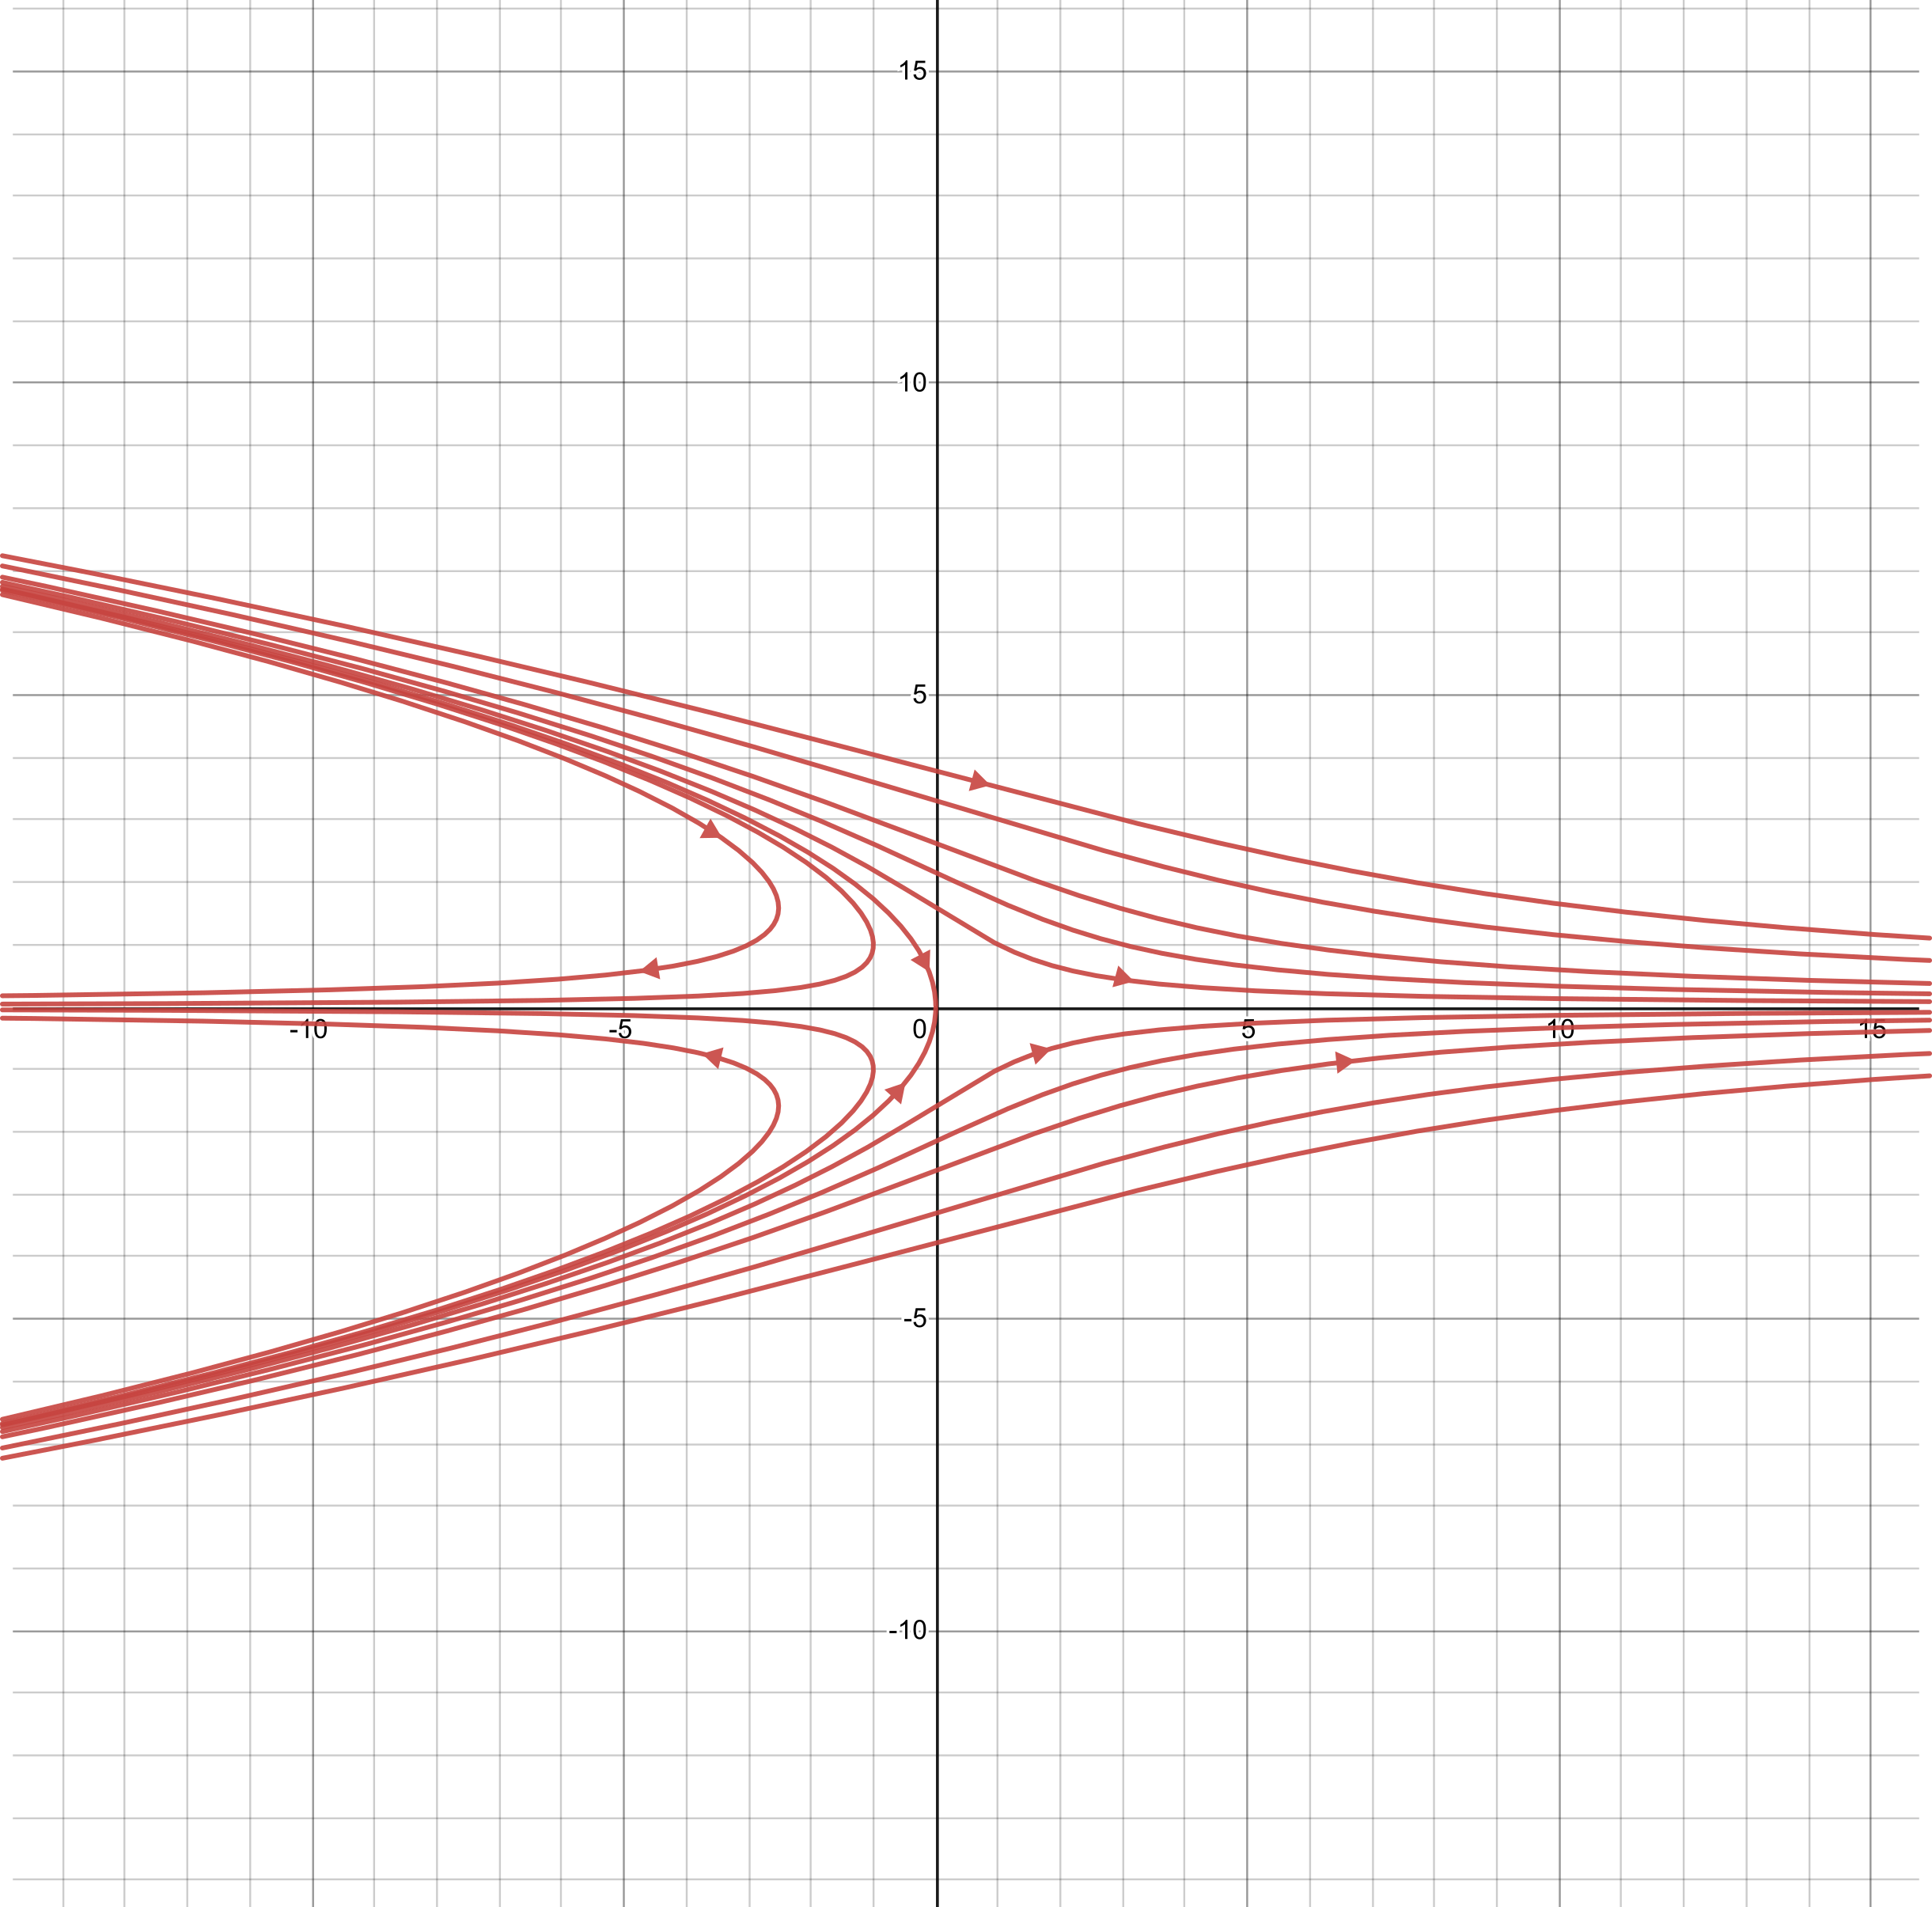
\includegraphics[scale=0.17]{Images/nonlinear_eg1.png}
    \caption{Phase portrait of non-linear system,  \href{https://www.desmos.com/calculator/hda60sxrdf}{source}}
    \label{fig:nonlinear-eg1}
\end{figure}

The parabola going through the origin is given by $x = -\frac{1}{3}y^2$. If our initial conditions lie on this parabola, we get
$$ x(t) = -\frac{y_0^2}{3} e^{-2t}, y(t) = y_0e^{t} $$
which draws out the above parabola.

Comparing phase portraits of the two systems, we can maybe convince ourselves of a certain similarity. The hope is that there is a way of `translating' one to the other (this is after all exactly what the homeomorphism would do). In fact in this case we can check that the change of variables given by
$$ T(x, y) = \left( x + \frac{1}{3}y^2, y \right) $$
maps the flow of the linear system onto the non-linear one.
\begin{align*}
    T^{-1} e^{tA} T(x_0, y_0) &= T^{-1} e^{tA} \left( x_0 + \frac{1}{3} y_0^2, y_0 \right)\\
    &= T^{-1}\left( e^t \left(x_0 + \frac{1}{3} y_0^2 \right), y_0 e^{-t} \right)\\
    &= \left( e^t \left(x_0 + \frac{1}{3} y_0^2 \right) - \frac{y_0^2}{3}e^{-2t}, y_0e^{-t} \right)
\end{align*}
which we know is exactly the flow of the non-linear system. In this case, the map $T$ linearised the system globally and was a diffeomorphism. Most of the time, this is not the case; usually, we only get local homeomorphisms as we see in the following example.

\subsubsection{Example 3}
Suppose 
$$ \matrix{x\\y}' = \matrix{\frac{1}{2} & -1\\1 & \frac{1}{2}} \matrix{x\\y} - \frac{1}{2}(x^2 + y^2) \matrix{x\\y} $$
Once again we see that the (only) steady state is at the origin and we can easily find that the differential at the origin is
$$ A := Df(0, 0) = \matrix{\frac{1}{2} & -1\\1 & \frac{1}{2}} $$
thus the linearisation is given by
$$ e^{tA} = e^{\frac{t}{2}} \matrix{\cos t & -\sin t\\ \sin t & \cos t} $$
Hence we conclude that the linearised system is a (counterclockwise) unstable spiral. 

With a slight change of variables, we will be able to see the qualitative behaviour of the non-linear system more easily. In particular, we will change to polar coordinates, $x(t) = r \cos \theta, y(t) = r \sin \theta$. Using some combinations of the product and chain rules, we find
\begin{align*}
    x' &= r' \cos\theta - r (\sin \theta) \theta'\\
    y' &= r' \sin \theta + r(\cos \theta) \theta'
\end{align*}
Multiplying and rearranging things appropriately, we get
\begin{align*}
    x x' + y y' = r r'\\
    -x'y + y'x = r^2 \theta'
\end{align*}
Therefore
$$ r' = \frac{1}{r} (xx' + y y') $$
where upon substituting things from the given ODE, we find 
$$ r' = \frac{1}{2} r - \frac{1}{2} r^3 $$
Similarly we find
$$ \theta' = \frac{1}{r^2} (-x'y + y'x) = 1 $$

We see that $r$ is stable when $r = 0, 1$ or $-1$. Obviously $r$ cannot be negative and we are ignoring the case of $r = 0$ (polar coordinates don't work here anyway and we've divided by $r$ too many times to give that a go), so the only interesting case is when $r = 1$. In this case, the solution is given by the unit circle since $\theta$ is a simple linear function.

Note that when $0 < r < 1$, $r' > 0$ thus $r$ is increasing and when $r > 1$, we have $r' < 0$ so $r$ is decreasing. Thus solutions that begin inside the unit circle grow towards it and solutions that begin outside decay towards it. 

% TODO: Add diagram of solution to spiral

Certainly then we cannot get a global homeomorphism to a linear system because no linear system has dynamics where it grows near the origin but shrinks far away from it. However we can get a local homeomorphism around the origin. Let $\Phi$ be the flow for the non-linear system and $\Psi$ the flow for the linearised system. Fix some $r_0  < 1$. Then for every $x \in B_{r_0}(0)$ there is some unique time $\tau$ such that $\Phi_t(x) \in B_{r_0}(0)$ (this is because the radius $r$ is increasing on such solutions). Thus we can think of $\tau$ as a function of the initial point $x$. Then we define the homeomorphism $h$ by $h(x) = \Psi_{-\tau}\Phi_{\tau}(x)$. We will show that this is a homeomorphism later.

% TODO: Add diagram of homeomorphism

\subsubsection{Example 4}
Consider the system
$$ \matrix{x\\y}' = \matrix{-y + \epsilon x(x^2 + y^2)\\x + \epsilon y(x^2 + y^2)} $$
As usual, the only equilibrium point is at the origin where the differential is
$$ Df(0, 0) = \matrix{0 & -1\\1 & 0} $$
The flow of the linearised system is therefore a center. In order to compare this with the original, non-linear system we write the original system in polar coordinates to get
$$ r' = \epsilon r^3, \theta' = 1 $$
Therefore when $\epsilon > 0$, we have a source at the origin and when $\epsilon  < 0$, we have a sink. Neither of these can be conjugate to a center (if they were, then we would conclude that a sink and source are conjugate and certainly no reasonable system of classification should consider such systems to be equivalent).

\subsubsection{Example 5}
Consider the system
$$ \matrix{x\\y}' = \matrix{x^2\\-y} $$
Then the linearisation around the equilibrium at the origin is
$$ Df(0, 0) = \matrix{0 & 0\\0 & -1} $$
In this case the linearisation produces an entire line of stability. However clearly this cannot be the case with the non-linear system, as at least one of $y'$ and $x'$ is non-zero everywhere (besides the origin). Indeed the origin is an unstable equilibrium since solutions on the x-axis for example always move to the right.

\subsection{Stability}\label{subsec:stability}
We've mentioned stability and instability quite a few times so far, without defining precisely what they mean (although we have an intuitive idea already). Let us remedy this now.
\begin{definition}[Stable/Unstable Equilbria]
Let $(\Phi_t)_{t \geq 0}$ be a dynamical system on a domain $D \subset \R^n$. Let $a$ be an equilibrium point. Then $a$ is said to be \textit{stable} if for every $\epsilon > 0$ there exists some $\delta > 0$ such that $|x - a| < \delta$ implies that $\sup_{t \geq 0} \left| \Phi_t(x) - a \right| < \epsilon$.

We can equivalently define stable equilibria in the language of open sets: an equilbrium point $a$ is said to be stable if for every neighbourhood $V$ of $a$ there is a neighbourhood $U$ of $a$ such that if $x \in U$ then $\Phi_t(x) \in V$ for all $t \geq 0$.

An equilibrium is said to be \textit{unstable} if it is not stable. This is equivalent to saying that there exists some $\epsilon > 0$ and a sequence $(x_j)_{j \in \N}$ in $D$ that converges to $a$ such that
$$ \sup_{t \geq 0} \left| \Phi_t(x_j) - a \right| \geq \epsilon $$
for all $j$.
\end{definition}
\begin{remark}
    The fact that $\Phi_t$ is a dynamical system means that $\Phi_0 = Id$ and $\Phi_{s + t} = \Phi_s \circ \Phi_t$. This is effectively the flow of a system. See \autoref{sec:dyn-systems} for more details.
\end{remark}
\begin{remark}
    In order to see why the above definition of instability is equivalent to the negation consider the following argument: if an equilibrium point is not stable then there is some $\epsilon > 0$ such that for all $\delta > 0$ we have some $x$ such that $\left| x - a \right| < \delta$ and $\sup_{t \geq 0} \left| \Phi_t(x_j) - a \right| \geq \epsilon$. Taking the $x_j$ to be the corresponding $x$ for $\delta = \frac{1}{j}$ we get the desired sequence.
\end{remark}
\begin{definition}
An equilibrium point $a$ is said to be asymptotically stable (or attractive) if $a$ is stable and there is some $\delta > 0$ such that $$\lim_{t \to \infty} \left| \Phi_t(x) - a \right| = 0$$
for all $\left| x - a \right| < \delta$.
\end{definition}
\begin{remark}
    The condition that $a$ be stable is necessary. You can construct counterexamples where $a$ is not stable but the second condition still holds.
\end{remark}

% TODO: Add diagram of counterexample

We have topological conjugacy between a system and its linearisation if hyperbolicity holds (which is to say, if the eigenvalues of the linearised system have non-zero real part). Although we will not prove this statement in general, we will state it and prove some special cases of it.

\begin{theorem}[Hartman-Grobman]\label{thm:hartman-grobman}
Consider $x' = f(x)$ for $f \in C^1$ and suppose $f(a) = 0$ (i.e. $x(t) \equiv a$ is an equilibrium). Let $A := Df(a)$ be hyperbolic. Let $\Phi_t$ be the dynamical system for the ODE and let $\Psi_t := e^{tA}$ be the dynamical system for the linearisation. Then, there is a neighbourhood $U$ of $a$ and neighbourhood $V$ of 0 and a homeomorphism $h: U \to V$ such that
$$ \Phi_t = h^{-1} \circ \Psi_t \circ h $$
provided $t$ is sufficiently small.
\end{theorem}

What can be learn by applying this theorem? Well for one thing, we can determine the stability or even asymptotic stability of equilibria. This is quite useful when analysing systems in the real world (gross). We also get the so-called \textit{stable/unstable curve theorem}, which roughly says that if the linearisation (of a planar system) has a saddle then so will the nonlinear system. In particular there will be two curves: the solutions starting on one curve will approach the origin as $t \to \infty$ (known as the stable curve) and solutions starting on the other curve will approach the origin as $t \to -\infty$ (known as the unstable curve). In \autoref{fig:nonlinear-eg1}, the stable curve is the `parabola' seen in the left half of the plane and the unstable curve is the $x$-axis (not drawn). This generalises to the stable/unstable manifold theorems for higher dimensional systems.

Unfortunately, the filter of topological conjugacy is quite broad. For example, all sinks are topologically conjugate to one another (as are all sources). Thus for example, you wouldn't be able to tell the difference between a spiral sink or a stable node. In some cases that is fine, in some cases it is not. We could perhaps say a bit more if we instead had that $h$ was a diffeomorphism. When can we get diffeomorphic conjugacy then? We need a certain non-resonance condition to hold.

Nevertheless, the Hartman-Grobman theorem is indicative of a more general principle, if the linearised system is `structurally stable' (in this instance, structurally stable means hyperbolic, although this may change in other contexts), then the non-linear system will look like the linear system, at least locally.  

We will only prove Hartman-Grobman in the special case when we have $n$ distinct, negative eigenvalues. But first we need the following lemma.
\begin{lemma} \label{lem:sink-solns}
Consider $x' = f(x)$ where $f$ is $C^1$ with an equilibrium at $a$. If $A := Df(a)$ has $n$ distinct, negative (hence real) eigenvalues. Then $a$ is asymptotically stable for the non-linear system (or equivalently, it is a sink).
\end{lemma}
\begin{proof}
Suppose $A = Df(a)$ has distinct, negative real eigenvalues. Then we claim that we can assume $A$ to be a diagonal matrix without loss of generality. This can be achieved by doing a change of basis if necessary. 

Suppose $D$ is the diagonalisation of $A$. In other words, there exists an invertible $T$ such that $A = T D T^{-1}$. Suppose $y$ is a solution to $y' = A y$. Then substituting $y = T \tilde{y}$, we find that $ (T \tilde{y})' = T \tilde{y}' = A T \tilde{y}$ or in other words $$\tilde{y}' = D \tilde{y}$$
We can similarly assume $a = 0$, by taking $\tilde{f}(x) = f(x + a)$ and considering $D \tilde{f}$ instead (then of course $D \tilde{f}(0) = Df(a)$).\\ 

Using the Taylor expansion, we have
$$ f(x) = f(0) + f'(0)x + \ol{o}(\left| x \right|) $$
where $\ol{o}(\left| x \right|)$ contains the higher order terms for the error (see \href{https://en.wikipedia.org/wiki/Big_O_notation#Little-o_notation}{Wikipedia} on little-o notation. If you want to see what exactly the remaining terms looks like, consider the \href{https://en.wikipedia.org/wiki/Taylor_series#Taylor_series_in_several_variables}{following} article). Thus the ODE reduces to
$$ x' = Ax + \ol{o}(\left| x \right|) $$
Now we define a function $L: \R^n \to \R$ where
$$ L(x) = \frac{1}{2}\left| x \right|^2 $$
Suppose $y$ is a solution to the linearisation. Intuitively, it is quite clear that the origin is asymptotically stable for the linearisation: we have a basis of eigenvectors and along each of these, the solutions decay. Since the general solution is a linear combination of these, it must decay as well. We will prove the statement formally using the technique of \textit{Lyapunov functions} (to be discussed shortly), a very useful technique that can be used in very general contexts.

We find that
\begin{align*}
    \frac{d}{dt} L(y(t)) = \frac{d}{dt} \left( \frac{1}{2} \left| y(t) \right|^2 \right) = y^{T} \cdot y' = y^{T} Ay = \lambda_1 y_1^2 + \dots + \lambda_n y_n^2 \leq \max\{ \lambda_1, \dots, \lambda_n \} \cdot |y|^2
\end{align*}
where $y^{T} \cdot y'$ refers to the dot product of the two vectors. In particular we find that if we let $c$ denote the above maximum, then
$$ \frac{d}{dt} L(y) \leq 2 c L(y) \leq c L(y) $$
where the second inequality holds because $c$ is negative. Then a consequence of (an easy case of) \hyperref[thm:easy-gronwall]{Grönwall} is that
$$ L(y(t)) \leq L(y(0)) e^{ct} $$
Since $c$ is negative, we know all such solutions decay.

Now suppose $x$ is a solution to the non-linear system. Then
\begin{align*}
    \frac{d}{dt} L(x(t)) = x^{T} \cdot x' &= x^{T} \left( Ax + \ol{o}(\left| x\right| \right)\\
    &\leq c \left| x \right|^2 + \ol{o}(\left| x \right|^2)
\end{align*}
We choose a neighbourhood $V$ of 0 so that for $x \in V$ we have
$$ |x|^2 \leq \frac{|c|}{2} = \frac{-c}{2} $$
Then by definition of little-o, we find that for $x(t) \in V$
\begin{align*}
    \frac{d}{dt} L(x(t)) \leq c \left|x(t) \right|^2 + \ol{o}(\left|x(t)\right|^2) \leq c \left|x(t) \right|^2 - \frac{c}{2} \left|x(t) \right|^2 = \frac{1}{2} c \left|x(t) \right|^2 = c L(x)
\end{align*}
By Grönwall again, what we find is that 
$$ L(x(t)) \leq L(x(0)) e^{ct} $$
Since $c$ is negative, this goes to 0 as $t \to \infty$. Since $L(x) = \frac{1}{2}|x|^2$, the same holds true for $|x|$ as well. Thus all solutions that start in $V$, approach the origin as $t \to \infty$, proving the claim that the origin is asymptotically stable for the non-linear system as well.
\end{proof}
Of course, the fact that the two flows are sinks does not (immediately) show that they are conjugate. We will do so shortly. However, before that a comment on the techniques used above. As mentioned, one of the key ingredients was the Lyapunov function.

\begin{definition}[Lyapunov functions]
Consider the differential equation $x' = f(x)$ with an equilibrium at $a$. Then a Lyapunov function is a real-valued, differentiable function on a neighbourhood of $a$ such that it is 0 on $a$ and positive everywhere else and also satisfies
$$ \frac{d}{dt} L(x(t)) \leq 0 $$
whenever $x(t)$ is a solution to the ODE.

If we have 
$$ \frac{d}{dt} L(x(t)) < 0 $$
for all non-constant solutions, then $L$ is said to be a strict Lyapunov function.
\end{definition}

In general it is difficult to find Lyapunov functions, however in certain cases this can be done by considering things like conservation of energy/momentum/etc (certainly any solution to an ODE in physics is going to satisfy the fact that energy is non-increasing with time).